\documentclass{report}
\usepackage{graphicx}
\usepackage{hyperref}


\begin{document}

% Pagina di Copertina
\begin{titlepage}
    \centering
    \vspace*{\fill}
    \Huge \textbf{THESIS TITLE}
    \vspace{2cm} 
    
    \Large Lorenzo Ferrari

    \vspace{2cm} % Spazio aggiuntivo tra il nome e il nome dell'istituto
    
    \Large Università degli studi di Parma
    \par
    Three-year degree course in Computer Science
    
 
\end{titlepage}

%indice
\renewcommand{\contentsname}{Index}
\tableofcontents
    
    
    
    %overview 
    \chapter{Introduction}
    introduction and some stuff
    % Capitolo buffer overflow
    \section{Tooling}
    In this thesis i will use many tools such as: 
       \begin{itemize}
        \item[$\bullet$] pwndbg : pwndbg is a GDB plugin that makes debugging with GDB with a focus on features needed by low-level software developers, hardware hackers, reverse engineers, and developer exploitation.\newline
        \item[$\bullet$]pwntools: is a very powerful Python library created to make difficult things easy in exploit development.\newline
        Such as receiving program output contents, sending user input, sending bytes instead of letters, and much more.\newline
        \item[$\bullet$] ghidra or ida free: 
        ghidra is a free tool developed by the NSA used to decompile binary files.
        ida free is the free version of ida pro and is a cloud base decompiler, the free version works only for some architecture such as x8664.\newline
        both tools are used in the reverse engineering part.\newline
    \end{itemize}
    
    \chapter{Buffer Overflow vulnerability}
    \section{background} %---------------------fix this text ------------------
    Buffer overflow is a critical vulnerability that emerged around the 1970s and 1980s where it was 
    realized through research which leads the attacker to uncontrolled access to critical points of memory.\newline
    As the 1990s arrived the explosion of the Internet and its client-server infrastructure led large numbers of people to use buffer overflow.\newline
    Furthermore, in this period the first books were published explaining how buffer overflow works.\newline
    In the 2000s people wanted to defend themselves from these types of attacks and invented two types of mitigations:\newline
    \begin{itemize}
        \item[$\bullet$] ASLR (Address Space Layout Randomization)
        \item[$\bullet$] stack canary 
    \end{itemize}
    We will explain this mitigation later.\newline
    Between 2000s and 2010s even with the mitigations attackers managed to avoid them and still exploit buffer overflow vulnerability with technique called:\newline
        \begin{itemize}
        \item[$\bullet$] ROP (Return Oriented Programming)
        \item[$\bullet$] RET2LIBC (Return to Libc)
    \end{itemize}
    Even though vulnerability was born so many years ago it still is one of the biggest an dangerous vulnerablity.
    \clearpage
    %-----------------fix until here--------------------
    \section{How Buffer Overflow works}
    A buffer overflow occurs when the attacker can write more input than expected from the buffer, the overflow input exceeds in the memory in the location right after the buffer we are allocating, this could be very dangerous.\newline
    here's an example:
    \begin{verbatim}
    #include <iostream>
    
    int main() {
    
        char buff[30]; // buffer victim 
        printf(" insert your name: ");
        scanf("%50s",buff); 
        return 0;
    }
    \end{verbatim}
    In this example we can see a bad usage of a scanf function. In fact, this program has a char buffer with a size of 30, but the scanf function can read up to 50 chars.\newline 
    What happens if we insert more input than expected for the buffer?\newline
    State of the buffer before inserting input:\newline
    \begin{figure}[h]
    \centering
    \includegraphics[width=13cm]{Organigrammi.png}
    \caption{Empty stack}
    \label{fig:example_empty_buffer}
    \end{figure}
       \clearpage
    In the example, we can notice that we have our buffer instantiated.\newline
    I wrote the question marks instead of 0x0000000000000000 because this memory at the beginning of the program is instantiated for the program we are executing, but this memory had previously been used in other contexts.\newline
    Now we will try to insert the following paylaod:
    \begin{verbatim}
        AAAAAAAAAAAAAAAAAAAAAAAAAAAAAAPPBBBBBBBBCCCCCCCC
    \end{verbatim}
    i used the "A" to fill the buffer "P" for the remaining buffer before RBP, "B" for overwriting the saved base pointer,
    C for overwriting the return address.
    this will cause a buffer overflow because when we get to the assembly instruction leave and ret it will not find the instruction 0x4343434343434343 and the program will receive a segmentation fault.
    \begin{figure}[h]
        \centering
        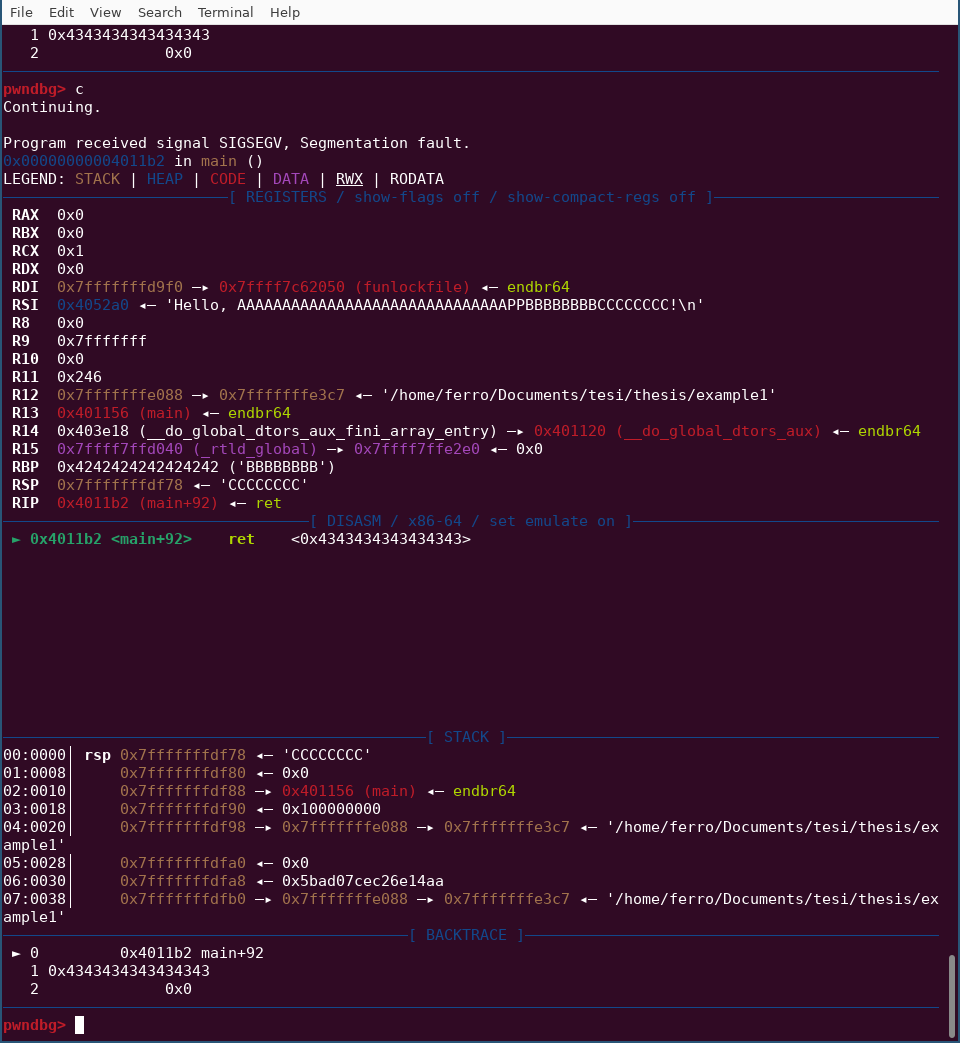
\includegraphics[width=0.9\linewidth]{example1.png}
        \caption{buffer overflow triggered}
        \label{fig:empty stack}
    \end{figure}
    \newpage
    
    This is how looks the stack after sending this payload:
    \begin{figure}[htbp]
        \centering
        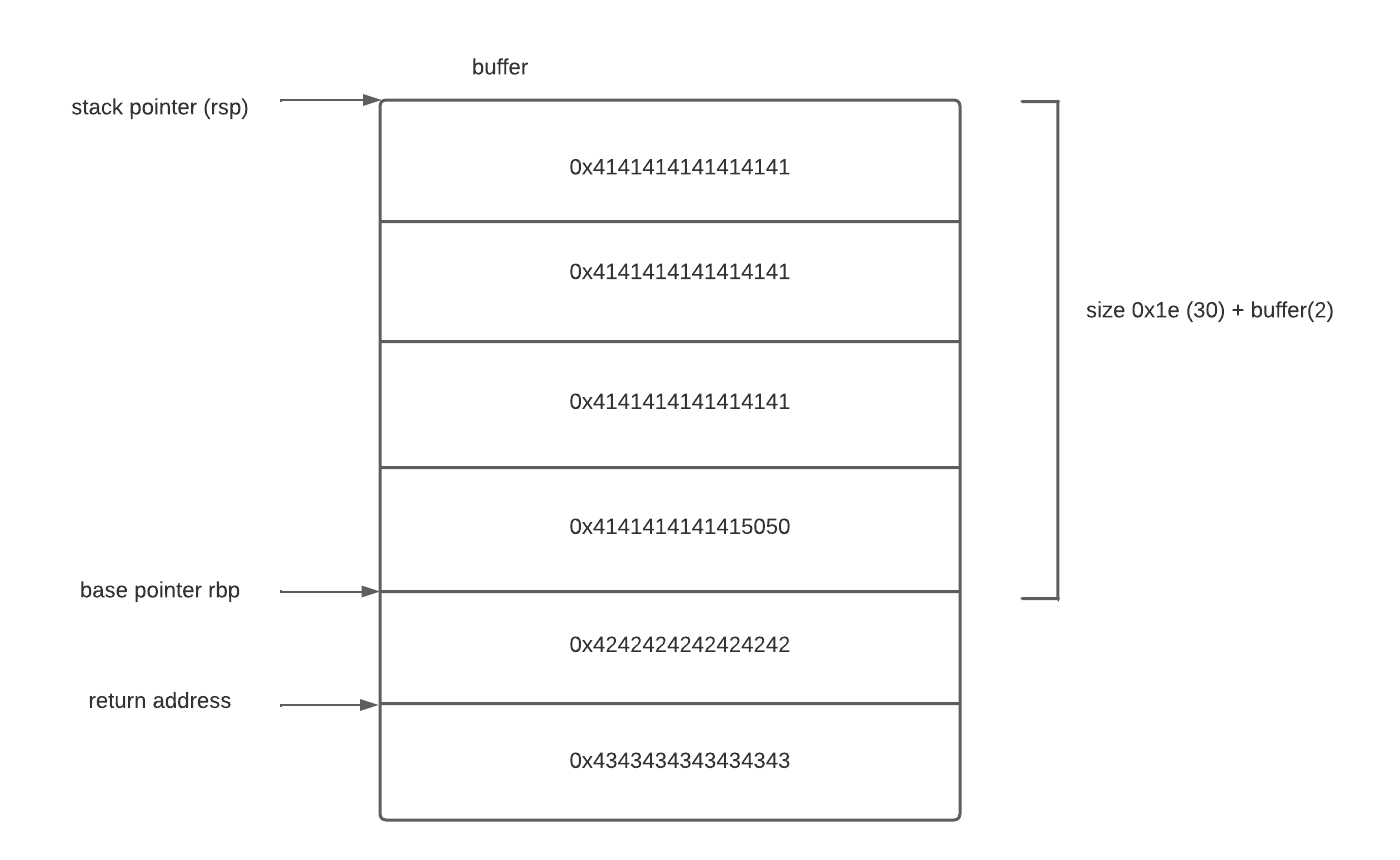
\includegraphics[width=1\linewidth]{stack_after_overflow.png}
        \caption{Stack after the overflow}
        \label{fig:stack w overflow}
    \end{figure}
    \clearpage
    \section{Mitigations against Buffer Overflow}
    \subsection{Stack Canary}
    The stack canary is a protection that was invented in the 90s to prevent a buffer overflow from occurring.
    It consists of generating a protection value, generated at run time and therefore different for each time a program is executed, but remains for the entire execution of the program.
    The stack canary is placed before important metadata such as the saved base pointer and return address.
    Before executing the epilogue of the function, the integrity of the value of the stack canary is checked. If this has been modified or tampered with, the program will end immediately with the following exit code:
    \begin{verbatim}
    *** stack smashing detected ***: terminated
    \end{verbatim}
    Compilers like gcc by default compile with stack canary, by analyzing the decompiled file the compiler will insert the following lines of code to insert the stack canary.\newline
    \begin{verbatim}
    if (local_10 != *(long *)(in_FS_OFFSET + 0x28)) {
                    /* WARNING: Subroutine does not return */
    __stack_chk_fail();
  }
    \end{verbatim}
    
    The name derives from a small historical note. In fact, the name "stack canary" was inspired by the technique used in coal mines.\newline
    To avoid entering an area of the mine with high levels of toxic gases, they would let a canary fly ahead.\newline
    If the canary died, passage was prohibited; otherwise, they could pass.
    \clearpage
    Following is the photo of the stack extracted from GDB. As we can see, I inserted two commands:
    \begin{itemize}
      \item \hspace{1em} canary: This command shows the possible canaries of this code.
      \item \hspace{1em} stack 20: This command shows 20 stack instances.
    \end{itemize}
    As we can see, at address 0x7fffffffdf68, we have the value 0xe1509a30995e5f00, which is our stack canary.
    \begin{figure}
        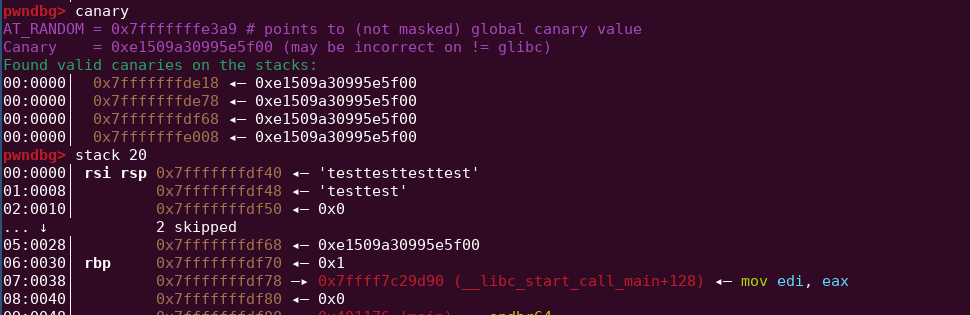
\includegraphics[width=1.3\linewidth]{photo_of_the_stack_with_canary.png}
        \caption{ stack canary on gdb }
        \label{fig:  photo stack canary}
    \end{figure}
    \clearpage
    \subsection{ASLR}
    ASLR stands for Address Space Layout Randomization and is a technique they invented to protect operating systems from memory attacks.\newline
    In fact ASLR has the task of randomizing sections of memory such as heap stacks and shared libraries every time a program or operating system is launched.\newline
    ASLR with the stack canary seen previously and PIE that we will see later are mitigations mainly developed to avoid buffer overflow, in fact ASLR for example avoids us from jumping into memory locations that would be in fixed positions if it were not for this mitigation, and it avoids many attacks.\newline
    ASLR can randomize memory segments between a range of:
    \begin{verbatim} 
    2^8(256) to  2^16(65536)
    \end{verbatim}
    on the linux kernel we can check the level of randomization with the following command:
    \begin{verbatim}
    cat /proc/sys/kernel/randomize_va_space
    2
    \end{verbatim}
    the result of the command is 2 this indicate that we have maximum number of randomization in my personal linux kernel.\newline
    Follows a photo that explain how aslr works.
    \begin{figure}[h]
        \centering
        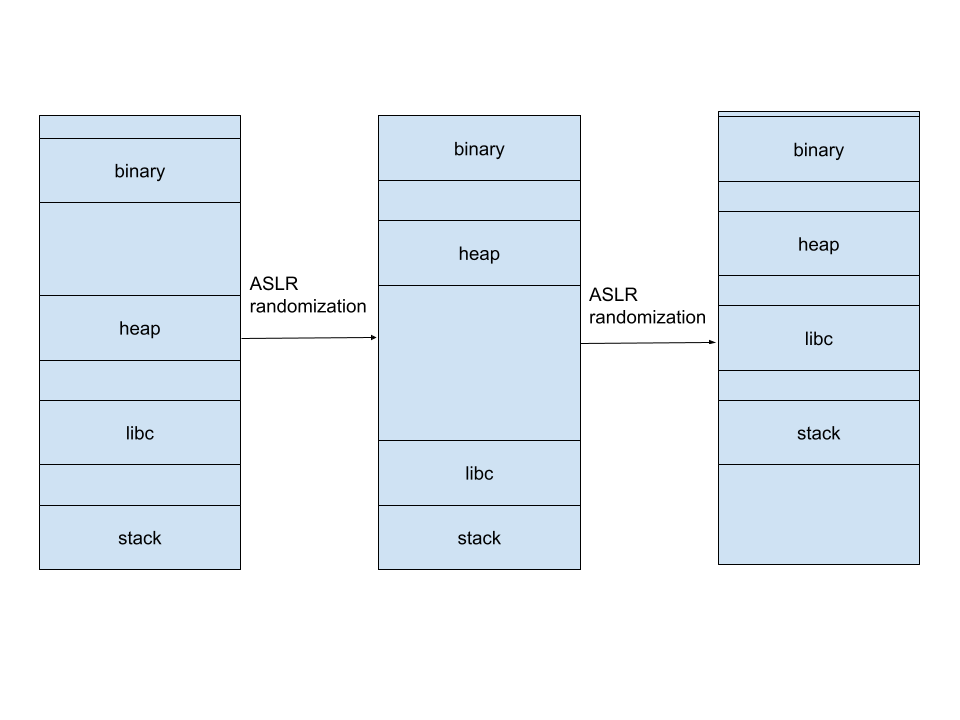
\includegraphics[width=0.8\linewidth]{aslr_explanation.png}
        \caption{ASLR}
        \label{fig:aslr }
    \end{figure}
    \clearpage
    \subsection{PIE}
    PIE stands for Position Independent Executable and is very similar to ASLR, in fact it follows the same concept as ASLR but with the binary assembly memory region.\newline
    As can be interpreted from the name Position Independent gives the possibility for a binary to be loaded and executed in memory at arbitrary addresses, this means that the program data instead of referring to addresses in fixed memory are referenced through the use of an offset random to the current position where it is loaded plus the offset.
    
    \begin{table}[h] % Utilizzo [b] per posizionare la tabella in fondo alla pagina
      \centering
      \begin{tabular}{|c|c|c|c|}
        \hline
        ASLR  & PIE & Binary Address & Libc Address \\
        \hline
        disable & disable  & 0x400000 & 0x7ffff7d86000 \\
        disable & disable  & 0x400000 & 0x7ffff7d86000\\
        disable & activated   & 0×555555554000 & 0x7ffff7d86000 \\
        disable & activated   & 0×555555554000 & 0x7ffff7d86000 \\
        activated  & disable  &  0x400000 & 0x7fe7833eb000 \\
        activated  & disable  &  0x400000& 0x7f1a44191000 \\
        activated  & activated   & 0×555555554000 & 0x7f29d6ebd000 \\
        activated  & activated   & 0×555555554000 & 0x7f7d008a0000 \\
        \hline
      \end{tabular}
    \end{table}
    \clearpage

    \section{How to exploit a buffer overflow and demonstration of a challenge}
    In this chapter I will explain the techniques used to exploit a buffer overflow and demonstrate how the techniques work with an example of an exploit.\newline
    As a demonstration I used a challenge proposed as training in preparation for the national competition.\newline
    I found and decided to present the following challenge because it includes the bypass of all mitigations and an exploitation technique that is still very effective.\newline
        The challenge is called terminator and two files are attached:

    \begin{itemize}
        \item[$\bullet$] file terminator ELF  
        \item[$\bullet$] libc with which they compiled that binary
    \end{itemize}
    \clearpage
    
    \subsection{Plan and organization of steps to carry out a challenge}
    When it comes to finding bugs in real-world applications or solving cybersecurity challenges, I like to divide the work into four main points: \newline
    \begin{itemize}
        \item[Step 1:] understand the environment.
        \item[Step 2:] reverse engineering.
        \item[Step 3:] understand which mitigations are.
        \item[Step 4:] write the exploit and test it.
    \end{itemize}

    \subsection{Understand the envirnoment}
    launching the command "file terminator"  we have the first information such as:\newline
    \begin{itemize}
        \item[$\bullet$] terminator is obviously a 64 bit x86-64 elf file.
        \item[$\bullet$] the binary is not stripped, this is positive because it implies that we will have debug symbols and in the reverse engineering phase it helps us a lot .
    \end{itemize}
    \subsection{Reverse Engineering}
    this is one of the most important and complicated phases, in fact from a binary file using tools such as IDA or Ghidra which interpret binary files and decompile them to make this phase easier.\newline
    Certainly, even with very powerful tools like these, the decompiled code will never be as clean as the original code.\newline
    In fact this phase involves an interpretation of the code through the decompiled code and the assembly that is shown.
    I decide to show a challenge with a very simple.
    I decided to show a challenge that has a simple reverse engineering part because the topic of the thesis is the exploitation phase.
    In fact we come across the following function which contains two critical bugs:\newline
    \clearpage
    \begin{figure}[h]
        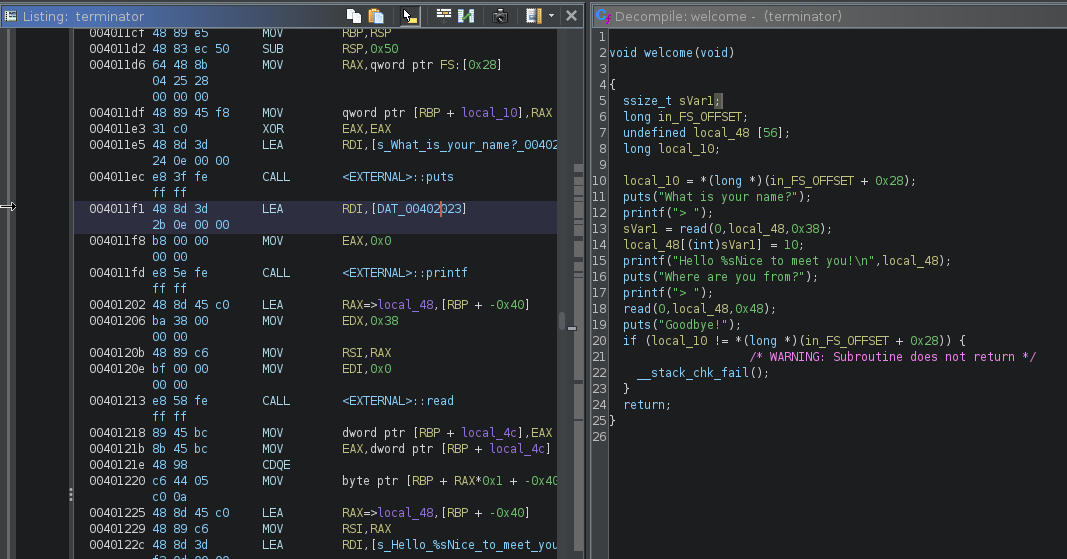
\includegraphics[width=1.3\linewidth]{terminator_rev.png}
        \caption{victim function on ghidra}
        \label{fig:rev_terminator}
    \end{figure}
    As we can see the decompiled version does not interpret the names of the variables and the types, in this specific case the reverse engineering part is simple but can usually take several hours, after a small adaptation the code we interpreted is the following:\newline
    \begin{figure}
        \centering
        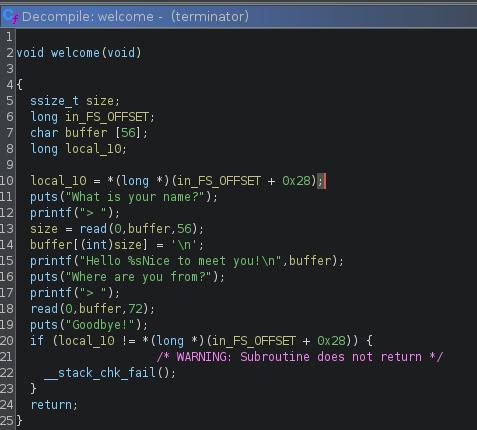
\includegraphics[width=1\linewidth]{terminator_rev2.png}
        \caption{victim function adapted}
        \label{fig:enter-label}
    \end{figure}

    \clearpage
        From this code we can interpret two critical bugs and one mitigation.\newline
    Initially a char buffer of size fifty six is instantiated, some prints are made and then we encounter the first bug.\newline
    The read function, as we can read from the manual, reads the number of bytes indicated within the function, in this specific case fifty six and does not add the null byte by default, in fact the programmer added it manually in the position that reflects the bytes read , however causing an off by one because it will put the null byte in the next byte at the end of the buffer, overwriting the first least significant byte of the next address.\newline
    vulnerable code:\newline
    \begin{verbatim} 
        char buffer [56];
        size = read(0,buffer,56);  
        buffer[(int)size] = '\n';
    \end{verbatim}
    The second critical bug is a buffer overflow where the provenance is requested, in fact it uses the same name buffer to save the provenance.
    Since the buffer is fifty-six characters long and the read has the number of bytes it will read set to seventy-two characters, this undoubtedly causes a buffer overflow of as many as fourteen characters.
    vulnerable code:\newline
    \begin{verbatim} 
    char buffer [56];
    read(0,buffer,72);
    \end{verbatim}
    Finally, from this function we can understand something that we would have analyzed later but realizing it previously already makes us aware of a potential problem.\newline
    In fact, from the decompiled code we find the code used by the compiler to insert the canary stack, which will prevent us from doing buffer overflows without first leaking the canary stack.\newline
    vulnerable code:
    \begin{verbatim} 
    if (local_10 != *(long *)(in_FS_OFFSET + 0x28)) {
                        /* WARNING: Subroutine does not return */
        __stack_chk_fail();
    }
    \end{verbatim}
    
    \clearpage
    \subsection{Understand which mitigations are active}
To understand the mitigations the pwntools library help us, in fact there is a feature that allows us to check the mitigations only with the following command:
    \begin{verbatim}
        checksec terminator                                     
[*] '/home/ferro/Downloads/terminator'
    Arch:     amd64-64-little
    RELRO:    Full RELRO
    Stack:    Canary found
    NX:       NX enabled
    PIE:      No PIE (0x400000)
    \end{verbatim}
    And the checksec command shows that we have a amd64-64-little that stand for x86-64 infrastructure, we have also Full RELRO that means we cant overwrite any plt and got section infact that memory is mapped as read only section, is not important for this specific exploit but in other exploitation techniques can be a big obstacle to bypass.\newline
    Than we have stack canary, we have already saw the canary code in the reverse engineering step, that confirm the presence of the canary, this will make our life difficult in the exploitation part.\newline
    Furthermore we have NX enabled so we cant execute shellcode directly in the stack.\newline
    And finally a good news we haven't PIE so the program data wont be randomize.\newline
    \subsection{Write the exploit and test it}
    \subsubsection{Leak canary and Base Pointer}
    The first step I did in the exploit is find the stack canary and save the base pointer because would be very useful later.
    The first overflow is perfect for our work, in fact if we look in the decompiled code we can see how the name input produces a bug, an off by one and allows us to overwrite the first byte of the canary stack, a feature of the canary stack is that the first three nibbles and therefore the first and a half bytes are always zero.\newline
    In fact the printf always prints up to the string terminator or null byte, this is the reason why the stack canary being after the name buffer will not be printed because the first byte is always a null byte.\newline
    But what happens if we overwrite the first byte of the canary with off by one?  
    \newpage
    exploit code to leak the canary:
    \begin{verbatim} 
    io.sendafter(b">", b"A"*56) # sending after char ">" 56*A 
    io.recvuntil(b'Hello '+ b'A'*56) #recive the output until HelloAAAA....A
    canary=io.recv(8) # save the canary  
    svb=io.recvuntil(b'Nice' , drop=True) 
    canary=b"\x00"+canary[1:8] # fixing the byte we overwrite to leak the canary
    real_canary=u64(canary[0:8]) #conver the canary to unsigned 64 bit 
    real_svb=u64(svb.ljust(8,b'\x00')) #convert the save base poiter to unsigned 64 bit
    log.info(f"leaked canary: {hex(real_canary)}") #stampo il canary
    log.info(f"leaked save base pointer: {hex(real_svb)}") #stampo il svp
    \end{verbatim}
    sendafter recvuntil are all pwntools functions that allow in the case of sendafter to send input bytes (in this case fifty-six A),
    recvuntil instead allows you to receive the program output.\newline
    \begin{figure}[h]
        \centering
        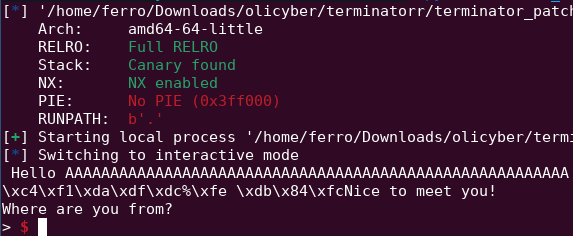
\includegraphics[width=1.3\linewidth]{leaked_canary_terminator.png}
        \caption{Enter Caption}
        \label{fig:leaked the canary in this function}
    \end{figure}
    
    As we can deduce from the image in the left shell after our A the stack canary and the save base pointer are printed, and you can see that the off by one was successful in fact the last byte of the canary instead of being \textbackslash x00 is \textbackslash x0a indicating \textbackslash n. \newline
    \clearpage
    Following is an image that explains the state of the stack after the off by one.\newline
    \begin{figure}[h]
        \centering
        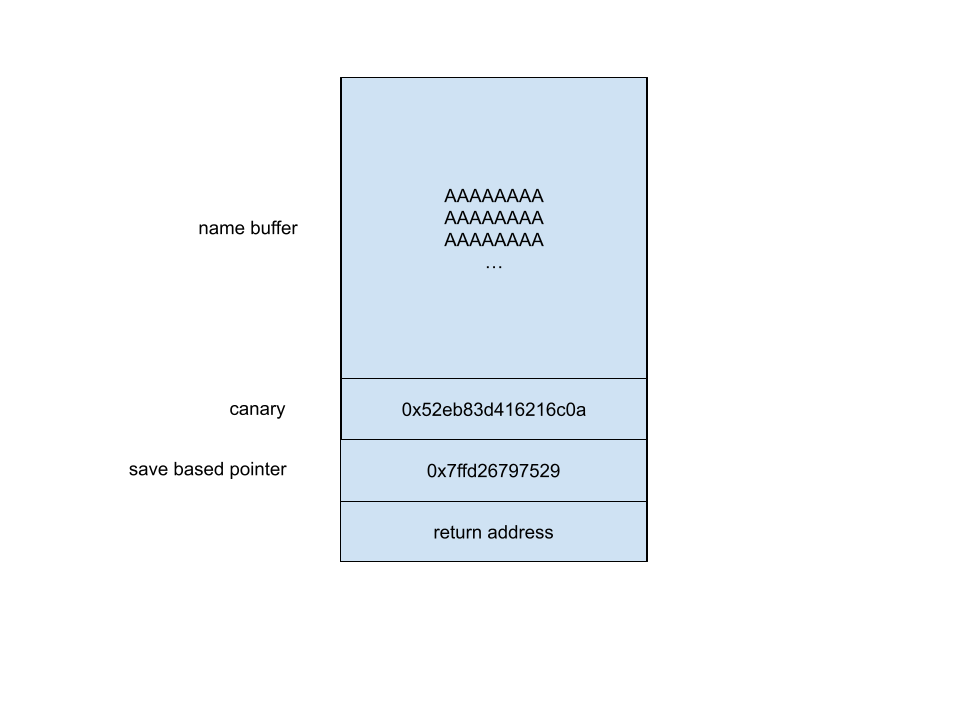
\includegraphics[width=1\linewidth]{draw_terminator_stack_canaryleak.png}
        \caption{stack status after off by one}
        \label{fig:stack terminator}
    \end{figure}
    As you can see the initial canary address 0x52eb83d416216c000
    was overwritten in the last byte and became 0x52eb83d416216c0a.
    The printf not encountering null bytes either in the contents of the stack canary or in the contents of the save base pointer will print both.\newline
    \subsubsection{Stack Pivoting and ASLR bypass}
    Now that we have the stack canary and the base pointer leak, we can move on to the part of the exploit that allows us to execute commands remotely.\newline
    Having NX as a mitigation we cannot write and execute shellcode on the stack so we will write a ROP chain.
    A ROP chain consists of searching inside our binary for assembly instructions which, when chained together, allow us to make syscalls that interest us.\newline
    \clearpage
    We have a tool that helps us search for gadgets called ropper.\newline
    \begin{verbatim}
    shell command used to find gadgets.
    ~/home/ferro/Downloads/terminator ropper --file=terminator
    \end{verbatim}
    This command will give us more than a hundred instructions as output, following is a photo of the section of the most interesting ones.\newline
    \begin{figure}[h]
        \centering
        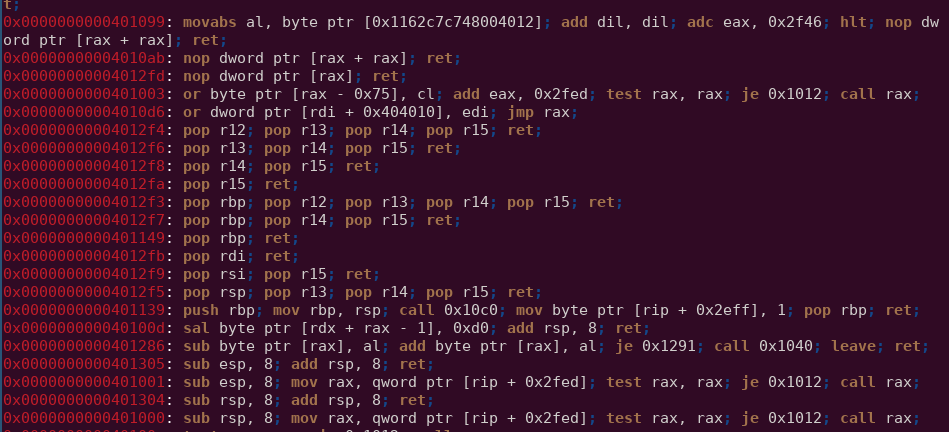
\includegraphics[width=1.2\linewidth]{rop_gadget.png}
        \caption{ropper result}
        \label{fig:ropper}
    \end{figure}
    
    At this point we can actually try to pop a shell with a rop chain and do remote command execution, but we would encounter two main problems.\newline
    \begin{itemize}
        \item[Problem 1:] We don't have enough space after the overflow to perform a rop chain.
        \item[Problem 2:] We don't have the base of the libc to bypass aslr.
    \end{itemize}
    So there are two solution: \newline
    \begin{itemize}
        \item[Solution 1:] Perform a stack pivoting attack.
        \item[Solution 2:] Leak  the libc address.
    \end{itemize}
    \clearpage
    \paragraph{Stack Pivoting}

    When we don't have enough space for the rop chain we can perform an attack called stack pivoting, it consist in manipulating the stack to enlarge the stack that we have available. \newline
    Basically we fake the rsp register to  enlarge the stack, there are many ways to perform a stack pivoting, we will find out my version later.\newline
    \paragraph{Leak the Libc base}
    To leak the base address of libc we will perform a puts of an got fuction address and after the leak, we will calculate the base of the libc doing :\newline
    \begin{verbatim}
        base Libc = address function with ASLR - fuction address with out ASLR  
    \end{verbatim}
    Follow the exploit code.\newline.
    \begin{verbatim}
                
        pop_rdi=0x4012fb
        puts1=0x84420      
        payload2=flat(
             p64(pop_rdi),#address of pop rdi
             p64(exe.got.puts),#address of got puts fucnion
             p64(exe.sym.puts),#address that will actualy print the got puts addres
             p64(0x00401292), #ret 
             p64(exe.sym.main),#calling main again
             b'A'*16,#fill the remaining space of the buffer
             p64(real_canary), #send the canary to bypass the canary mitigation
             p64(target_bp), #send the target base pointe    
        )
        io.sendafter(b">", payload2)
    \end{verbatim}
        
    Here is the exploit as we can see at the beginning I saved the addresses of pop rdi which is very useful because it allows us to populate the contents of the syscall, then the address of puts without base and then calculate it later.\newline
    Subsequently I will write the rop that will allow me to do stack pivoting and leak the puts address to calculate the base of the libc.\newline

    DEVO RI EXPLOITARE LA CHALLENGE NON RICORDO DELLE COSE LOL

    \clearpage
    %capitolo heap overflow 
    \chapter{Heap Overflow Vulnerability}
    \section{Background}
        This attack was first documented in 2005 in a paper called malloc maleficarum, where 5 techniques that are still usable today called: 
       \begin{itemize}
        \item[$\bullet$] house of force
        \item[$\bullet$] house of spirit
        \item[$\bullet$] house of prime  
        \item[$\bullet$] house of lore 
        \item[$\bullet$] house of mind
    \end{itemize}

    have been explained, in this chapter we will talk about the most famous, house of force which includes a bug called heap overflow.
    \clearpage
    
    \section{Malloc internal}
    The next bug that I will show, as can be understood from the name, concerns another section of memory such as the heap that works differently than the stack.\newline
    The heap known as Dynamic memory is a memory that is used for dynamic allocation, this is useful because you don't need to care about the size and the life time of the object. \newline
    Furthermore the heap in languages as C is manipulated from the user through functions as malloc() calloc() that permit you to create heap memory section usually called chunk, and free() to free your memory.\newline
     \begin{verbatim}
         void *a = malloc(8);
     \end{verbatim}

    \begin{figure}[htbp]
        \centering
        \includegraphics[width=1.2\linewidth]{image.png}
        \caption{chunk in gdb}
        \label{fig:enter-label}
    \end{figure}
    
    Immagine to have this line of code, what is happening in the heap memory?\newline
    The heap will create this chunk where the first quad-word is 0x20 that represent the size of the chunk, 0x20 is the minimum size for a chunk, and the pointer to the chunk will be the next quad word "0x4ce770".\newline

    So we can deduce that the heap saves data such as the size inline directly on the heap, like the stack does for base pointers, etc.\newline
    The last nibble of the size field is 0x1, is used to represent flags, in this case the least significant bit is set indicating prev\_insue.\newline
    The prev\_inuse flags indicate, if the previous contiguous chunk is used will be set to 1 otherwise 0. \newline
    Last thing i want to talk about malloc internal is the top chunk.\newline
    Malloc treats that as yet unused heap memory as a single large chunk called top chunk.\newline
    In Fact every time we request memory from a malloc or calloc function we are stealing a part of the top chunk.\newline
    The value indicated in gdb previously is the remaining space of the heap memory.\newline
    In many glibc version the top chunk value hasn't any type of integrity check, this will be the point of the heap overflow.\newline
    \clearpage
    
    \section{How it works a Heap Overflow}
    As explained previously, malloc(), calloc() and realloc() are libc functions that allow you to create portions of dynamic memory called chunks into which data can be inserted dynamically.
    But if these features are used incorrectly, there is a possibility that an attacker will exploit these mistakes to create critical attacks.
    \begin{verbatim}
        void *malloc(size_t size);
        void *calloc(size_t nmemb, size_t size);
        void *realloc(void *ptr, size_t size);
    \end{verbatim}
    These are the definitions of malloc calloc and realloc from the linux manual, as you can see all the functions require a size, which is often the cause of many heap overflows.
    The following is vulnerable code that shows a misuse of size within these functions:
    \begin{verbatim}
        #include <stdio.h>
        #include <stdlib.h>
        void setup() {
          setbuf(stdin, NULL);
          setbuf(stderr, NULL);
          setbuf(stdout, NULL);
        }
        
        int main(){
            setup();
            puts("Insert your name: ");
        
            char *buf = malloc(100);
            if (buf == NULL) {
                fprintf(stderr, "Error malloc failed, NO INPUT");
                return 1;
            }
            scanf("%s", buf);
            printf("hello %s\n", buf);
        
            free(buf);
            return 0;
        }
    \end{verbatim}
    This code contains a critical bug, as can be seen when user input is entered, scanf is not used correctly, in fact the correct use is to specify \%n-1s in the format string where n is the size of the buffer and minus one is used because scanf add a null byte as a terminator.
    \clearpage
    Consequently if the user enters more than 96 characters there will be a heap overflow.\newline
    Potential payload and heap analysis:
    \begin{verbatim}
        AAAAAAAAAAAAAAAAAAAAAAAAAAAAAAAAAAAAAAAAAAAAAAAAAAAAAAA
        AAAAAAAAAAAAAAAAAAAAAAAAAAAAAAAAAAAAAAAAAAAAAAAAAAAAAAA
    \end{verbatim}
        \begin{figure}[htbp]
        \centering
        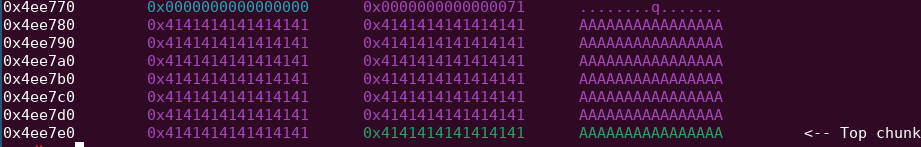
\includegraphics[width=1\linewidth]{heap_overflow.png}
        \caption{Heap overflow viewed in gdb }
        \label{fig:enter-label}
    \end{figure}
    How can we analyze the chunk that we have allocated "buf" is allocated previously compared to the value of the top chunk, so by performing an overflow we will overwrite the value of the top chunk with the value 0x4141414141414141
    the heap will think that the size of the remaining heap will be an arbitrary number.\newline
    At this point the program will not crash because at the time I am writing this thesis no type of integrity check on the size of the top chunk has been implemented, this allows us to create arbitrary write.
    \clearpage
    \paragraph{Craft arbitrary write}
    Basically in the world of exploitation we always try to have arbitrary writes and arbitrary reads.\newline
    Arbitrary read permit us to read addresses that allow us to bypass mitigations such asth aslr, canary. \newline
    Arbitrary writes to overwrite addresses that lead us to have remote command execution.
    In the case of the example shown above we have no print source so crafting an arbitrary read is impossible but in larger and more complicated systems they can be found. \newline
    But we have an arbitrary writing source, in fact we can overwrite the size of the top chunk making it giant and managing to overwrite the libraries and stack sections so as to overwrite sensitive data.
    \begin{figure}[htbp]
        \centering
        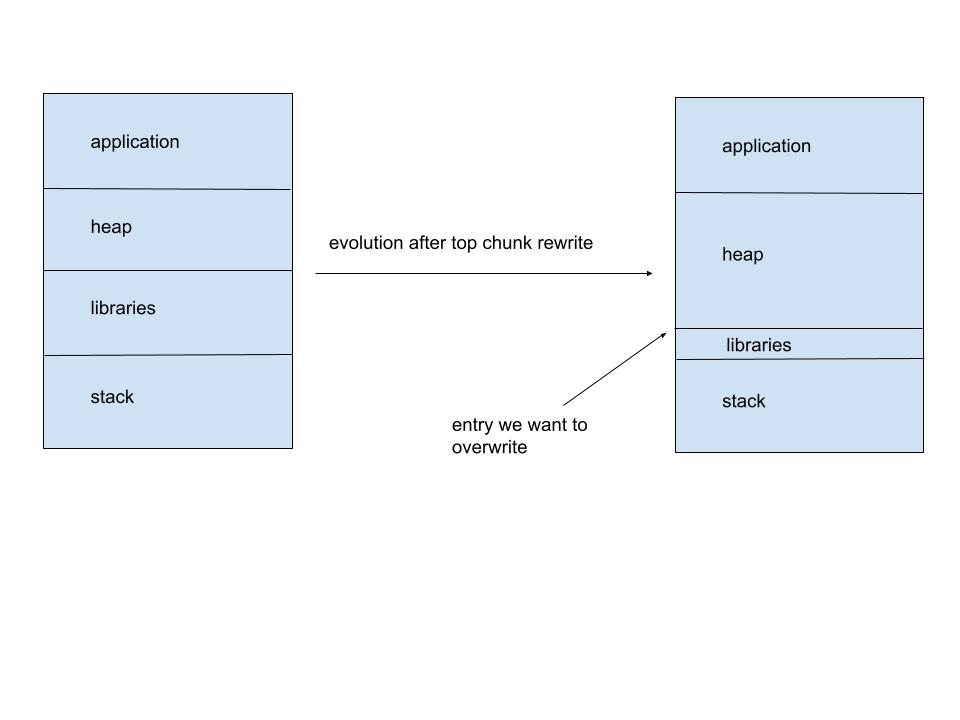
\includegraphics[width=1\linewidth]{heap_trasformation.jpg}
        \caption{heap after overwriting top chunk}
        \label{fig:enter-label}
    \end{figure}
    \clearpage
    
    \section{overview challenge and attack planning}
    In this section we will analyze a challenge that I solved during the csaw qualifier competition, a competition organized by an American team where the top 8 teams went to New York to play the finals.\newline
    In the challenge we will analyze there is a heap overflow bug, the name of the challenge is phrack. \newline
    
    \clearpage
    \section{exploit analisys}
    to be continued
    \clearpage
    %capitolo double free
    \chapter{Double Free Vulnerability}
    \section{How it works a Double Free}
    to be continued    
    \clearpage
    \section{overview challenge and attack planning}
    to be continued
    \clearpage
    \section{exploit analisys}
    to be continued
    \clearpage
    % capitolo conclusioni
    \chapter{Conclusion}
    to be continued
    \section{online references}
    \href{https://it.wikipedia.org/wiki/Home_page}{wikipedia}
    
    \clearpage
\end{document}
